% Options for packages loaded elsewhere
\PassOptionsToPackage{unicode}{hyperref}
\PassOptionsToPackage{hyphens}{url}
\PassOptionsToPackage{dvipsnames,svgnames,x11names}{xcolor}
%
\documentclass[
  10pt,
  a4paper,
  onecolumn]{article}

\usepackage{amsmath,amssymb}
\usepackage{iftex}
\ifPDFTeX
  \usepackage[T1]{fontenc}
  \usepackage[utf8]{inputenc}
  \usepackage{textcomp} % provide euro and other symbols
\else % if luatex or xetex
  \usepackage{unicode-math}
  \defaultfontfeatures{Scale=MatchLowercase}
  \defaultfontfeatures[\rmfamily]{Ligatures=TeX,Scale=1}
\fi
\usepackage{lmodern}
\ifPDFTeX\else  
    % xetex/luatex font selection
\fi
% Use upquote if available, for straight quotes in verbatim environments
\IfFileExists{upquote.sty}{\usepackage{upquote}}{}
\IfFileExists{microtype.sty}{% use microtype if available
  \usepackage[]{microtype}
  \UseMicrotypeSet[protrusion]{basicmath} % disable protrusion for tt fonts
}{}
\makeatletter
\@ifundefined{KOMAClassName}{% if non-KOMA class
  \IfFileExists{parskip.sty}{%
    \usepackage{parskip}
  }{% else
    \setlength{\parindent}{0pt}
    \setlength{\parskip}{6pt plus 2pt minus 1pt}}
}{% if KOMA class
  \KOMAoptions{parskip=half}}
\makeatother
\usepackage{xcolor}
\usepackage[top=18mm,bottom=15mm,left=5mm,right=5mm]{geometry}
\usepackage{soul}
\setlength{\emergencystretch}{3em} % prevent overfull lines
\setcounter{secnumdepth}{-\maxdimen} % remove section numbering
% Make \paragraph and \subparagraph free-standing
\ifx\paragraph\undefined\else
  \let\oldparagraph\paragraph
  \renewcommand{\paragraph}[1]{\oldparagraph{#1}\mbox{}}
\fi
\ifx\subparagraph\undefined\else
  \let\oldsubparagraph\subparagraph
  \renewcommand{\subparagraph}[1]{\oldsubparagraph{#1}\mbox{}}
\fi


\providecommand{\tightlist}{%
  \setlength{\itemsep}{0pt}\setlength{\parskip}{0pt}}\usepackage{longtable,booktabs,array}
\usepackage{calc} % for calculating minipage widths
% Correct order of tables after \paragraph or \subparagraph
\usepackage{etoolbox}
\makeatletter
\patchcmd\longtable{\par}{\if@noskipsec\mbox{}\fi\par}{}{}
\makeatother
% Allow footnotes in longtable head/foot
\IfFileExists{footnotehyper.sty}{\usepackage{footnotehyper}}{\usepackage{footnote}}
\makesavenoteenv{longtable}
\usepackage{graphicx}
\makeatletter
\def\maxwidth{\ifdim\Gin@nat@width>\linewidth\linewidth\else\Gin@nat@width\fi}
\def\maxheight{\ifdim\Gin@nat@height>\textheight\textheight\else\Gin@nat@height\fi}
\makeatother
% Scale images if necessary, so that they will not overflow the page
% margins by default, and it is still possible to overwrite the defaults
% using explicit options in \includegraphics[width, height, ...]{}
\setkeys{Gin}{width=\maxwidth,height=\maxheight,keepaspectratio}
% Set default figure placement to htbp
\makeatletter
\def\fps@figure{htbp}
\makeatother

\usepackage{amssymb, amsmath}

\makeatletter
\renewcommand*\env@matrix[1][\arraystretch]{%
  \edef\arraystretch{#1}%
  \hskip -\arraycolsep
  \let\@ifnextchar\new@ifnextchar
  \array{*\c@MaxMatrixCols c}}
\makeatother


\numberwithin{equation}{section}

\usepackage[utf8]{inputenc}
\usepackage{lastpage} % counts all the pages, used in footer
\usepackage{hyperref}

\usepackage{tikz}
\usetikzlibrary{arrows.meta}

% TIKS TEMPLATES
\tikzset{
dot/.style = {circle, fill, minimum size=#1,
              inner sep=0pt, outer sep=0pt},
dot/.default = 4pt % size of the circle diameter 
}
\tikzset{
sum/.style = {circle, draw=black, inner sep=-0.5pt}
}

\tikzset{
box/.style = {rectangle, draw=black, minimum width = #1},
box/.default = 1cm, % size of the circle diameter 
}

\usepackage{gensymb}

\usepackage{xfrac}

\setlength\columnsep{20pt}

% Package for enabling colors (colorful output)
\usepackage[dvipsnames]{xcolor}
\definecolor{darkgreen}{HTML}{014f32}

% Icons - http://mirrors.ctan.org/fonts/fontawesome5/doc/fontawesome5.pdf
\usepackage{fontawesome5}

% removes spacing in display math
\usepackage[nodisplayskipstretch]{setspace}

\usepackage{tabularx}

% Font Configuration
\usepackage{lmodern}
\renewcommand{\familydefault}{\sfdefault}
\usepackage{cmbright}
\usepackage[scaled=0.9]{inconsolata}

% 
\usepackage{fancyhdr}

\renewcommand{\headrulewidth}{1pt}
\renewcommand{\footrulewidth}{1pt}

\pagestyle{fancy}
\fancyhead{} % clear all header fields
\makeatletter
\fancyhead[R]{\@title}
\makeatother
\fancyhead[L]{HSLU T\&A}
\fancyfoot{} % clear all footer fields
\fancyfoot[C]{\thepage\ / \pageref{LastPage}}
\fancyfoot[R]{RGT}
\fancyfoot[L]{\today}

% introduces conditions environment to create nice equation parameter descriptions
\usepackage{array}

\newenvironment{conditions}
  {\par\vspace{\abovedisplayskip}\noindent\begin{tabular}{>{$}l<{$} @{${}:{}$} l}}
  {\end{tabular}\par\vspace{\belowdisplayskip}}
  

% Used for pandoc code block generations.
% Introduces breaklines for overflowing code blocks, by defining the Highlighting environment with breakline & symbol.
% Don't know what commandchars does :)
\usepackage{fvextra}
\DefineVerbatimEnvironment{Highlighting}{Verbatim}{
  breaklines=true,
  breakanywhere=true,
  breaksymbolleft={\textcolor{gray}{\scriptsize\ensuremath\hookrightarrow}},
  commandchars=\\\{\}
}



\let\paragraph\oldparagraph
\let\subparagraph\oldsubparagraph

\usepackage{xhfill}
\usepackage[explicit]{titlesec}
\renewcommand{\paragraph}[1]{\oldparagraph{#1}\mbox{}\par}

\titleformat{\section}[block]{\bfseries\Large}{\thetitle.}{3mm}{#1\space\xrfill[0.6ex]{1pt}}


\usepackage{pdfpages}
\usepackage{float}
\makeatletter
\let\oldlt\longtable
\let\endoldlt\endlongtable
\def\longtable{\@ifnextchar[\longtable@i \longtable@ii}
\def\longtable@i[#1]{\begin{figure}[H]
\onecolumn
\begin{minipage}{0.5\textwidth}
\oldlt[#1]
}
\def\longtable@ii{\begin{figure}[H]
\onecolumn
\begin{minipage}{0.5\textwidth}
\oldlt
}
\def\endlongtable{\endoldlt
\end{minipage}
\twocolumn
\end{figure}}
\makeatother
\usepackage[nswissgerman]{babel}
\makeatletter
\@ifpackageloaded{tcolorbox}{}{\usepackage[skins,breakable]{tcolorbox}}
\@ifpackageloaded{fontawesome5}{}{\usepackage{fontawesome5}}
\definecolor{quarto-callout-color}{HTML}{909090}
\definecolor{quarto-callout-note-color}{HTML}{0758E5}
\definecolor{quarto-callout-important-color}{HTML}{CC1914}
\definecolor{quarto-callout-warning-color}{HTML}{EB9113}
\definecolor{quarto-callout-tip-color}{HTML}{00A047}
\definecolor{quarto-callout-caution-color}{HTML}{FC5300}
\definecolor{quarto-callout-color-frame}{HTML}{acacac}
\definecolor{quarto-callout-note-color-frame}{HTML}{4582ec}
\definecolor{quarto-callout-important-color-frame}{HTML}{d9534f}
\definecolor{quarto-callout-warning-color-frame}{HTML}{f0ad4e}
\definecolor{quarto-callout-tip-color-frame}{HTML}{02b875}
\definecolor{quarto-callout-caution-color-frame}{HTML}{fd7e14}
\makeatother
\makeatletter
\makeatother
\makeatletter
\makeatother
\makeatletter
\@ifpackageloaded{caption}{}{\usepackage{caption}}
\AtBeginDocument{%
\ifdefined\contentsname
  \renewcommand*\contentsname{Inhaltsverzeichnis}
\else
  \newcommand\contentsname{Inhaltsverzeichnis}
\fi
\ifdefined\listfigurename
  \renewcommand*\listfigurename{Abbildungsverzeichnis}
\else
  \newcommand\listfigurename{Abbildungsverzeichnis}
\fi
\ifdefined\listtablename
  \renewcommand*\listtablename{Tabellenverzeichnis}
\else
  \newcommand\listtablename{Tabellenverzeichnis}
\fi
\ifdefined\figurename
  \renewcommand*\figurename{Abbildung}
\else
  \newcommand\figurename{Abbildung}
\fi
\ifdefined\tablename
  \renewcommand*\tablename{Tabelle}
\else
  \newcommand\tablename{Tabelle}
\fi
}
\@ifpackageloaded{float}{}{\usepackage{float}}
\floatstyle{ruled}
\@ifundefined{c@chapter}{\newfloat{codelisting}{h}{lop}}{\newfloat{codelisting}{h}{lop}[chapter]}
\floatname{codelisting}{Listing}
\newcommand*\listoflistings{\listof{codelisting}{Listingverzeichnis}}
\makeatother
\makeatletter
\@ifpackageloaded{caption}{}{\usepackage{caption}}
\@ifpackageloaded{subcaption}{}{\usepackage{subcaption}}
\makeatother
\makeatletter
\@ifpackageloaded{tcolorbox}{}{\usepackage[skins,breakable]{tcolorbox}}
\makeatother
\makeatletter
\@ifundefined{shadecolor}{\definecolor{shadecolor}{rgb}{.97, .97, .97}}
\makeatother
\makeatletter
\@ifundefined{codebgcolor}{\definecolor{codebgcolor}{HTML}{f7f7f7}}
\makeatother
\makeatletter
\makeatother
\ifLuaTeX
  \usepackage{selnolig}  % disable illegal ligatures
\fi
\IfFileExists{bookmark.sty}{\usepackage{bookmark}}{\usepackage{hyperref}}
\IfFileExists{xurl.sty}{\usepackage{xurl}}{} % add URL line breaks if available
\urlstyle{same} % disable monospaced font for URLs
\hypersetup{
  pdftitle={Regelungstechnik},
  pdfauthor={Joel von Rotz},
  colorlinks=true,
  linkcolor={blue},
  filecolor={Maroon},
  citecolor={Blue},
  urlcolor={Blue},
  pdfcreator={LaTeX via pandoc}}

\title{Regelungstechnik}
\author{Joel von Rotz}
\date{Invalid Date}

\begin{document}
 % [START] title
 % [ELSE] beamer

\makeatletter
\begin{center}
  \vspace*{0.5cm}
  
  \textbf{\Huge \@title}\\
  \vspace{0.1cm}
  \textsf{\textit{\large Zusammenfassung}}
  
  \vspace{0.5cm}

  \textsf{\large \@author \hspace{0.3cm}\textbf{/}\hspace{0.3cm}\large \faGithub\space \href{https://github.com/joelvonrotz/bachelor-electrical-engineering/tree/main/semester\%204/summary/regelungstechnik}{Quelldateien}}
  

\end{center}
\makeatother

 % [END] beamer
 % [END] title
\ifdefined\Shaded\renewenvironment{Shaded}{\begin{tcolorbox}[breakable, sharp corners, enhanced, colback={codebgcolor}, boxrule=0pt, frame hidden, borderline west={3pt}{0pt}{shadecolor}]}{\end{tcolorbox}}\fi

\renewcommand*\contentsname{Inhaltsverzeichnis}
{
\hypersetup{linkcolor=}
\setcounter{tocdepth}{3}
\tableofcontents
}
\newpage

% keep this to have smaller code blocks
\ifdefined\Shaded\renewenvironment{Shaded}{\begin{tcolorbox}[
  colback={shadecolor},
  boxrule=0pt,
  left=3pt,
  right=3pt,
  top=3pt,
  bottom=3pt,
  frame hidden,
  enhanced,
  breakable
]}{\end{tcolorbox}}\fi

\hypertarget{systeme}{%
\section{Systeme}\label{systeme}}

\hypertarget{grundlegende-systeme}{%
\subsection{Grundlegende Systeme}\label{grundlegende-systeme}}

\hypertarget{regler-system}{%
\subsubsection{Regler System}\label{regler-system}}

\begin{center}
  \begin{tikzpicture}
  % Boxes
    \node[box, minimum height=0.8cm, inner sep=5pt] (regBox) at (-1.5,2) {Regler $C$};
    \node[box, minimum height=0.8cm, inner sep=5pt] (procBox) at (1,2) {Prozess $P$};

  % Node
    \node[sum] (sumPoint) at (-3,2) {+};
    \node (startNode) at (-4,2) {};
    \node[dot] (endDot) at (2.5,2) {};
    \node(endPoint) at (3.5,2) {};
    \node (interferencePoint) at (1,3) {};

  % Lines
    \draw[->] (startNode) -- node[above]{$r$} (sumPoint);
    \draw[->] (sumPoint) -- node[above]{$e$} (regBox);
    \draw[->] (regBox) -- node[above]{$u$} (procBox);
    \draw (procBox) -- (endDot);
    \draw[->] (endDot) -- node[above]{$y$} (endPoint);
    \draw[->] (endDot) -- (2.5,1) -- (-3,1) -- node[above left]{$-$} (sumPoint);
    \draw[->] (interferencePoint) -- node[above=2mm]{$v$} (procBox);
  \end{tikzpicture}
\end{center}

\begin{conditions}
  r & Führungsgrösse (Soll-Wert) \\
  e & Regelfehler \\
  u & Stell-/Steuergrösse \\
  y & Regelgrösse (Ist-Wert) \\
  v & Störgrösse
\end{conditions}

\hypertarget{geschlossenes-system}{%
\subsubsection{Geschlossenes System}\label{geschlossenes-system}}

\begin{center}
  \begin{tikzpicture}
  % Boxes
    \node[box, minimum height=0.8cm, inner sep=5pt] (regBox) at (-1.5,2) {Regler $C$};
    \node[box, minimum height=0.8cm, inner sep=5pt] (procBox) at (1,2) {Prozess $P$};

  % Node
    \node[dot] (endDot) at (2.5,2) {};
    \node(endPoint) at (3.5,2) {};

  % Lines
    \draw[-{>[scale=1.5]}] (regBox) -- (procBox);
    \draw (procBox) -- (endDot);
    \draw[-{>[scale=1.5]}] (endDot) -- (endPoint);
    \draw[-{>[scale=1.5]}] (endDot) -- (2.5,1) -- (-3,1) -- (-3,2) -- (regBox);
  \end{tikzpicture}
\end{center}

\hypertarget{offenes-system}{%
\subsubsection{Offenes System}\label{offenes-system}}

\begin{center}
  \begin{tikzpicture}
  % Boxes
    \node[box, minimum height=0.8cm, inner sep=5pt] (regBox) at (-1.5,2) {Regler $C$};
    \node[box, minimum height=0.8cm, inner sep=5pt] (procBox) at (1,2) {Prozess $P$};

  % Node
    \node(endPoint) at (3,2) {};
    \node(startPoint) at (-3.5,2) {};

  % Lines
    \draw[-{>[scale=1.5]}] (regBox) -- (procBox);
    \draw[-{>[scale=1.5]}] (procBox) -- (endPoint);
    \draw[-{>[scale=1.5]}] (startPoint) -- (regBox);
  \end{tikzpicture}
\end{center}

\begin{tcolorbox}[enhanced jigsaw, leftrule=.75mm, opacityback=0, left=2mm, arc=.35mm, breakable, coltitle=black, rightrule=.15mm, opacitybacktitle=0.6, titlerule=0mm, title=\textcolor{quarto-callout-important-color}{\faExclamation}\hspace{0.5em}{Schleifenübertragungsfunktion}, bottomtitle=1mm, colbacktitle=quarto-callout-important-color!10!white, colframe=quarto-callout-important-color-frame, colback=white, bottomrule=.15mm, toptitle=1mm, toprule=.15mm]

\[
L(s) = C(s)\cdot P(s)
\]

\end{tcolorbox}

\hypertarget{vorsteuerung}{%
\subsubsection{Vorsteuerung}\label{vorsteuerung}}

Mit einer Vorsteuerung kann die Regelungszeit gekürzt werden (kleinerer
Fehler zum Auskorrigieren).

\begin{figure}[H]

{\centering 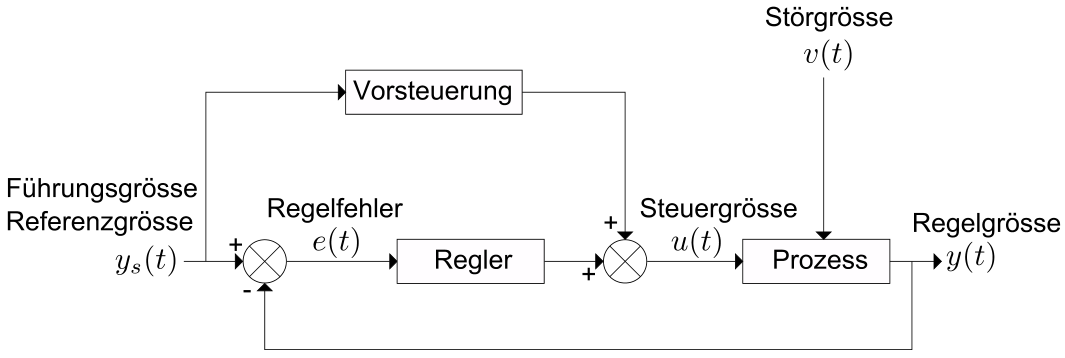
\includegraphics{images/paste-1.png}

}

\end{figure}

\hypertarget{minimalphasiges-system}{%
\subsection{Minimalphasiges System}\label{minimalphasiges-system}}

Liegen \ul{keine} Pole oder Nullstellen in der \ul{rechten Halbebene},
so spricht man von \textbf{minimalphasigen Systeme}. Amplituden- und
Phasengang stehen in einer direkten Beziehung zueinander. Es gilt
\textbf{nur bei minimalphasigen Systemen}:

\[
\angle{G}\approx\frac{\pi}{2}\cdot\frac{d{\log\lvert G\rvert}}{d{\log{\omega}}}
\]

Pro \(20\text{dB}\) Steigung oder Abfall beträgt die Phasenverschiebung
\(+90\degree\), respektive \(-90\degree\).

\hypertarget{fuxfchrungsverhalten}{%
\subsection{Führungsverhalten}\label{fuxfchrungsverhalten}}

\begin{figure}[H]

{\centering 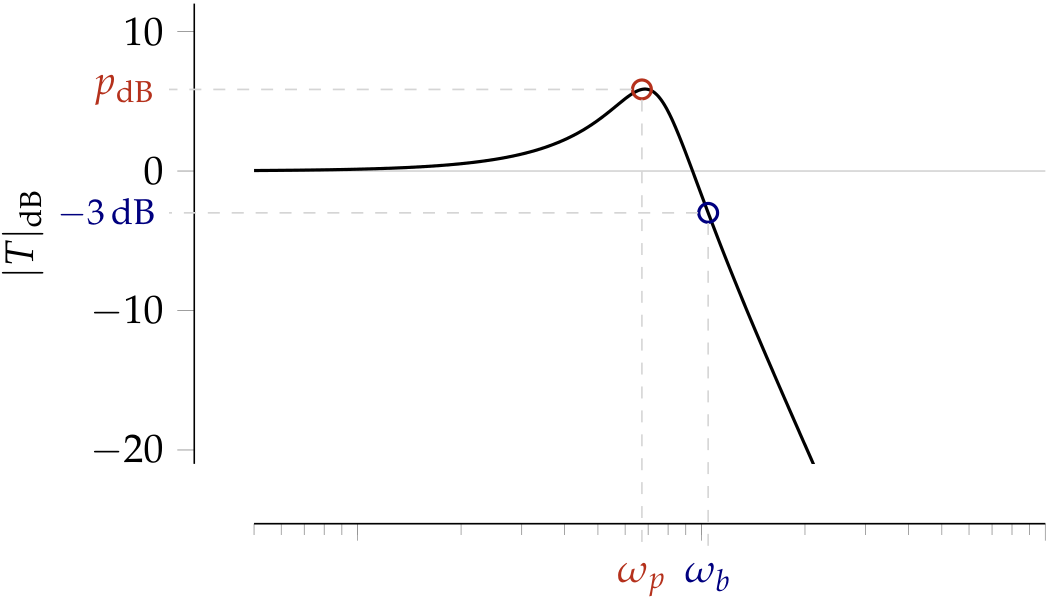
\includegraphics[width=6cm,height=\textheight]{images/paste-35.png}

}

\end{figure}

\[
G_{yr}=T=\frac{PC}{1+PC}\quad\text{und}\quad G_{ur}=CS=\frac{C}{1+PC}
\]

\hypertarget{merkmale}{%
\subsubsection{Merkmale}\label{merkmale}}

Das Führungsverhalten verfügt über vier Merkmale, welche für jedes
System betrachtet soll:

\begin{itemize}
\tightlist
\item
  \textbf{Stabilität}
\item
  \textbf{Statischer Fehler /} \textbf{stationäre Genauigkeit}
\item
  \textbf{Überschwingen}
\item
  \textbf{Schnelles Erreichen des stationären Wertes}
\end{itemize}

\textbf{Gutes Führungsverhalten}

\begin{figure}[H]

{\centering 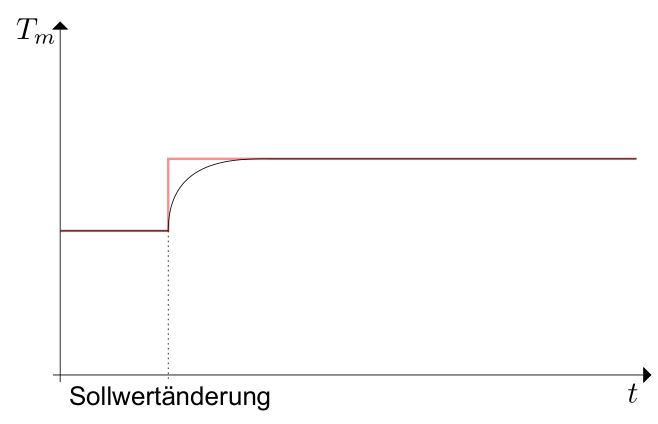
\includegraphics[width=6cm,height=\textheight]{images/fuhrungsverhalten/gutes_verhalten.png}

}

\end{figure}

\textbf{Instabilität}

\begin{figure}[H]

{\centering 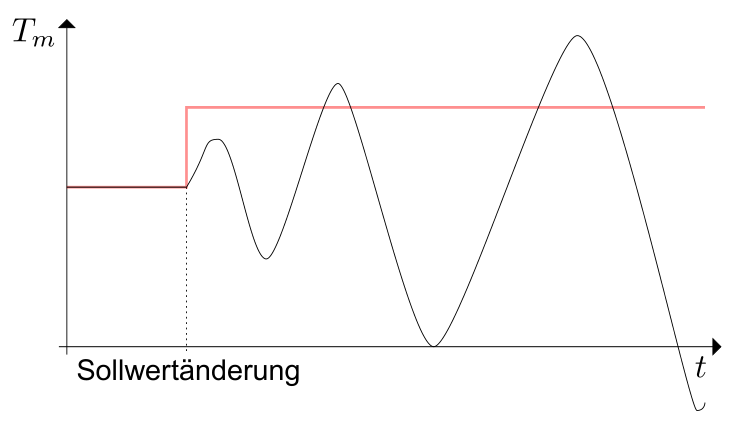
\includegraphics[width=6cm,height=\textheight]{images/fuhrungsverhalten/instabil.png}

}

\end{figure}

\textbf{Statischer Fehler /} \textbf{stationäre Ungenauigkeit}

\begin{figure}[H]

{\centering 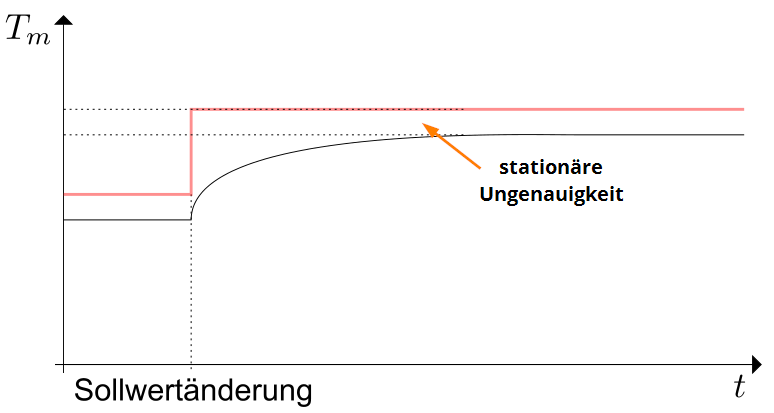
\includegraphics[width=6cm,height=\textheight]{images/fuhrungsverhalten/stationary.png}

}

\end{figure}

\textbf{Überschwingen}

\begin{figure}[H]

{\centering 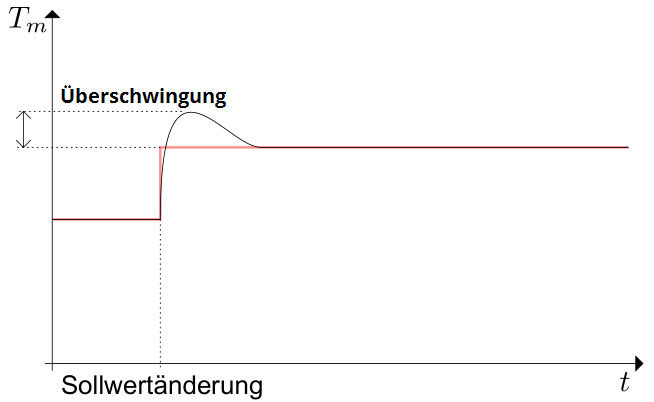
\includegraphics[width=6cm,height=\textheight]{images/fuhrungsverhalten/uberschwingung.png}

}

\end{figure}

\textbf{Langsames Erreichen des neuen stationären Wertes}

\begin{figure}[H]

{\centering 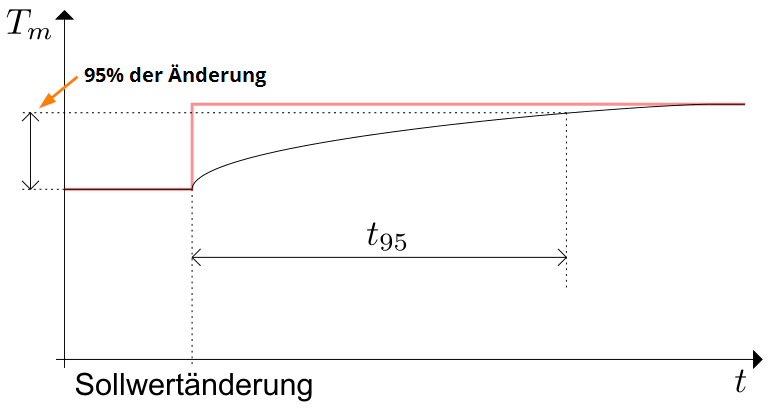
\includegraphics[width=6cm,height=\textheight]{images/fuhrungsverhalten/slow.png}

}

\end{figure}

\hypertarget{bleibende-fehler-bei-langsam-oder-nicht-uxe4ndernden-regelgruxf6ssen}{%
\subsubsection{Bleibende Fehler bei langsam oder nicht ändernden
Regelgrössen}\label{bleibende-fehler-bei-langsam-oder-nicht-uxe4ndernden-regelgruxf6ssen}}

Der bleibende Fehler bei sich langsam oder nicht ändernden
Führungssgrössen ergibt sich anhand des Verlaufs der
Übertragungsfunktion bei tiefen Frequenzen.

\[
G_{yr}\approx 1-e_0-e_1\cdot s-e_2\cdot s^2 - \cdots
\]

\[
e = e_0 \cdot r + e_1 \cdot \dot{r}+e_2\cdot \ddot{r}+\cdots
\]

\begin{figure}[H]

{\centering 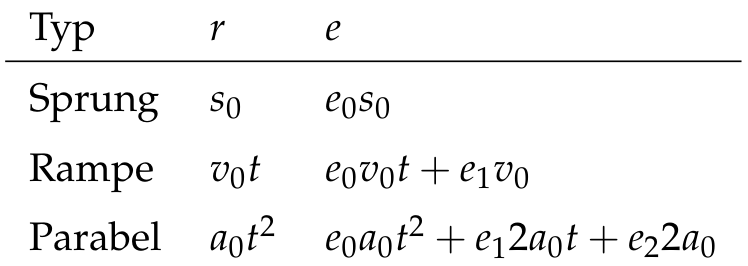
\includegraphics[width=5cm,height=1.8cm]{images/paste-37.png}

}

\end{figure}

\begin{tcolorbox}[enhanced jigsaw, leftrule=.75mm, opacityback=0, left=2mm, arc=.35mm, breakable, coltitle=black, rightrule=.15mm, opacitybacktitle=0.6, titlerule=0mm, title=\textcolor{quarto-callout-note-color}{\faInfo}\hspace{0.5em}{Stationärer Fehler}, bottomtitle=1mm, colbacktitle=quarto-callout-note-color!10!white, colframe=quarto-callout-note-color-frame, colback=white, bottomrule=.15mm, toptitle=1mm, toprule=.15mm]

Bei Rampe: \(e_0 = 0\qquad\) Bei Parabel \(e_0 = e_1 = 0\)

\end{tcolorbox}

\hypertarget{stuxf6rverhalten}{%
\subsection{Störverhalten}\label{stuxf6rverhalten}}

\[
G_{er}(s)=\frac{E(s)}{R(s)}
\]

\hypertarget{merkmale-1}{%
\subsubsection{Merkmale}\label{merkmale-1}}

Das Störverhlaten verfügt ebenfalls über vier Merkmale, welche für jedes
System betrachtet soll:

\begin{itemize}
\tightlist
\item
  \textbf{Stabilität}
\item
  \textbf{Statischer Fehler /} \textbf{stationäre Genauigkeit}
\item
  \textbf{Überschwingen}
\item
  \textbf{Schnelles Erreichen des stationären Wertes}.
\end{itemize}

\textbf{Gutes Störverhalten}

\begin{figure}[H]

{\centering 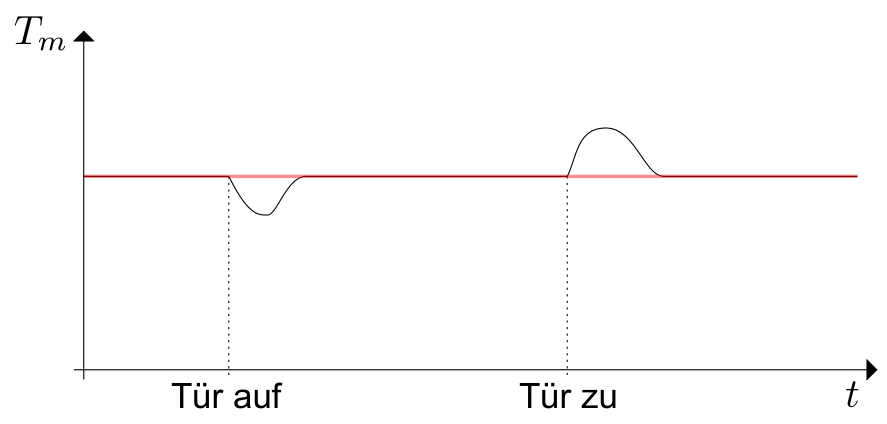
\includegraphics[width=6cm,height=\textheight]{images/storverhalten/gutes_verhalten.png}

}

\end{figure}

\textsuperscript{rot: Sollwert}

\textbf{Instabilität}

\begin{figure}[H]

{\centering 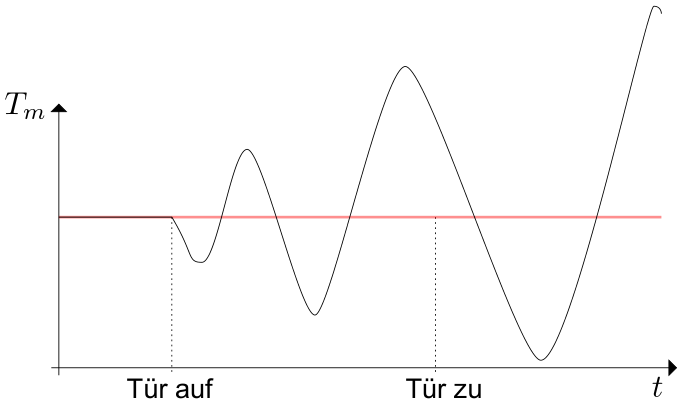
\includegraphics[width=6cm,height=\textheight]{images/storverhalten/storverhalten_stability.png}

}

\end{figure}

\textbf{Stationärer Fehler / Ungenauigkeit}

\begin{figure}[H]

{\centering 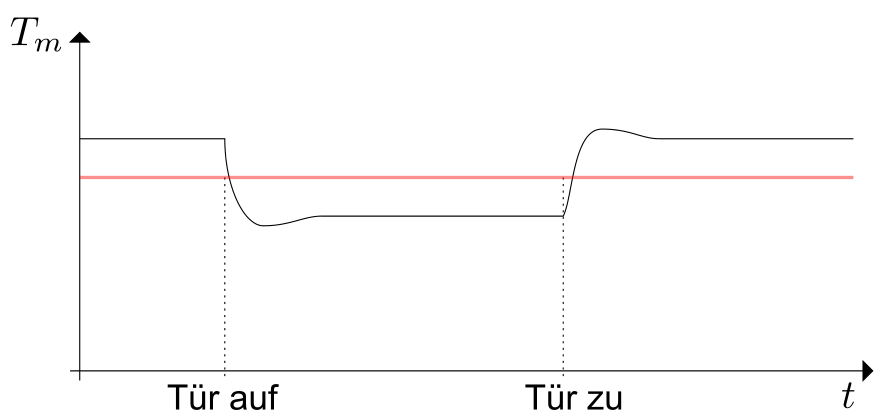
\includegraphics[width=6cm,height=\textheight]{images/storverhalten/storverhalten_stationary.png}

}

\end{figure}

\textbf{Überschwingen}

\begin{figure}[H]

{\centering 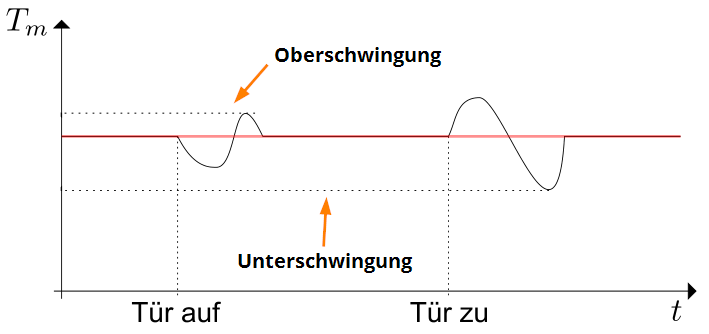
\includegraphics[width=6cm,height=\textheight]{images/storverhalten/uber_unterschwingung.png}

}

\end{figure}

\textbf{Langsames Erreichen des stationären Wertes}

\begin{figure}[H]

{\centering 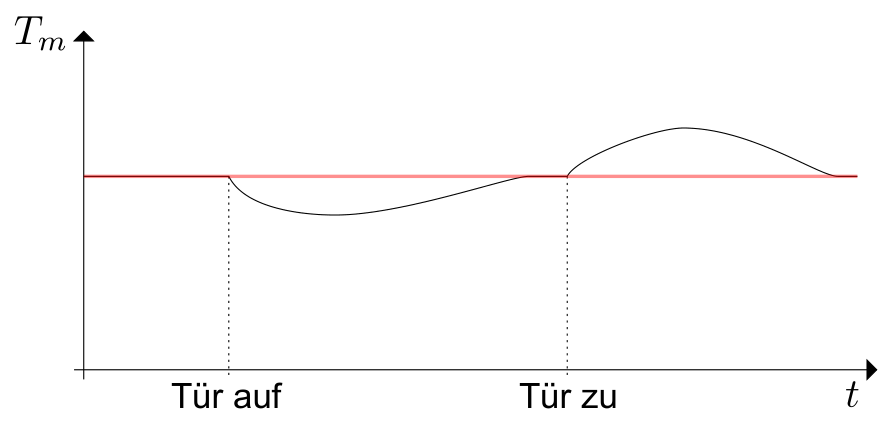
\includegraphics[width=6cm,height=\textheight]{images/storverhalten/slow.png}

}

\end{figure}

\hypertarget{darstellungsarten}{%
\section{Darstellungsarten}\label{darstellungsarten}}

\hypertarget{blockdiagrammalgebra}{%
\subsection{Blockdiagrammalgebra}\label{blockdiagrammalgebra}}

\hypertarget{verkettung}{%
\subsubsection{Verkettung}\label{verkettung}}

\begin{center}
\begin{tikzpicture}
    \node[box=0.8cm, minimum height=0.8cm] (sysG1) at (0,0) {$G_1$};
    \node[box=0.8cm, minimum height=0.8cm](sysG2) at (1.5,0) {$G_2$};
    \node[box=0.8cm, minimum height=0.8cm] (sysG12) at (0.75,-1) {$G_1G_2$};
    \node(start) at (-1.5,0) {};
    \node(end) at (3,0) {};
    \node(start2) at (-1,-1) {};
    \node(end2) at (2.5,-1) {};
    \draw[->]  (start2) edge node[above]{$u$} (sysG12);
    \draw[->]  (sysG12) edge node[above]{$y$} (end2);
    
    \draw[->]  (start) edge node[above]{$u$} (sysG1);
    \draw[->]  (sysG1) edge (sysG2);
    \draw[->]  (sysG2) edge node[above]{$y$}  (end);
    
\end{tikzpicture}
\end{center}

\[
y = G_2 ( G_1 \cdot u) = (G_1G_2)\cdot u
\]

\hypertarget{parallel}{%
\subsubsection{Parallel}\label{parallel}}

\begin{center}
\begin{tikzpicture}
    \node[box=0.8cm, minimum height=0.8cm] (sysG1) at (1,1.5) {$G_1$};
    \node[box=0.8cm, minimum height=0.8cm] (sysG2) at (1,0) {$G_2$};
    \node[box=0.8cm, minimum height=0.8cm] (sysG12) at (1,-1) {$G_1+G_2$};
    \node[dot] (dotStart) at (0,0.75) {};
    \node[sum] (sumEnd) at (2,0.75) {+};
    \node(start) at (-1.,0.75) {};
    \node(end) at (3,0.75) {};
    \node(start2) at (-1,-1) {};
    \node(end2) at (3,-1) {};
    \draw[->] (start2) edge node[above]{$u$} (sysG12);
    \draw[->] (sysG12) edge node[above]{$y$} (end2);
    
    \draw     (start) edge node[above]{$u$} (dotStart);
    \draw[->] (dotStart) |- (sysG1);
    \draw[->] (dotStart) |- (sysG2);
    \draw[->] (sysG1) -| (sumEnd);
    \draw[->] (sysG2) -| (sumEnd);
    \draw[->] (sumEnd) edge node[above]{$y$}  (end);
    
\end{tikzpicture}
\end{center}

\[
y = G_1\cdot u + G_1 \cdot u = (G_1 + G_2)\cdot u
\]

\hypertarget{ruxfcckkopplung}{%
\subsubsection{Rückkopplung}\label{ruxfcckkopplung}}

\begin{center}
\begin{tikzpicture}
    \node[sum] (sumStart) at (0,1) {$+$};
    \node[box=0.8cm, minimum height=0.8cm] (sysG) at (1.5,1) {$G$};
    \node[box=0.8cm, minimum height=0.8cm] (sysG12) at (1.25,-1) {$\frac{G}{1+G}$};
    \node(start) at (-1,1) {};
    \node(end) at (3.5,1) {};
    \node[dot] (endDot) at (2.5,1) {};
    \node(start2) at (-0.5,-1) {};
    \node(end2) at (3,-1) {};
    
    \draw[->]  (start2) edge node[above]{$r$} (sysG12);
    \draw[->]  (sysG12) edge node[above]{$y$} (end2);
    
    \draw[->]  (start) edge node[above]{$r$} (sumStart);
    \draw[->]  (sumStart) edge node[above]{$e$} (sysG);
    \draw      (sysG) edge (endDot);
    \draw[->]  (endDot) edge node[above]{$y$}  (end);
    
\draw[->] (endDot) -- (2.5,0) -- (0,0) -- node[above left]{$-$} (sumStart);
\end{tikzpicture}
\end{center}

\[
\begin{split}
y &= G\cdot e = G(r-y)\\
(1+G)\cdot y &= G\cdot r \\
y &= \underbrace{\frac{G}{1+G}}_{G_{yr}} \cdot r\\
\end{split}
\]

\hypertarget{regel-von-mason}{%
\subsubsection{Regel von Mason}\label{regel-von-mason}}

\[
G_{ij} = \frac{\sum_k P_k\cdot\Delta_k}{\Delta}
\]

\[
\begin{split}
P_k &= \text{Vorwärtspfad } k\\
\Delta = 1 &- \small{\Sigma\text{ aller Loops}} \\
           &+ \small{\Sigma\text{ aller Produkte 2er Loops, die sich nicht berühren}} \\
           &- \small{\Sigma\text{ aller Produkte 3er Loops, die sich nicht berühren}} \\
           &+ \cdots \\
\Delta_k = 1 &- \small{\Sigma\text{ aller Loops, die $P_k$ nicht berühren}} \\
             &+ \small{\Sigma\text{ aller Produkte 2er Loops, die $P_k$ \& sich nicht berühren}} \\
             &- \small{\Sigma\text{ aller Produkte 3er Loops, die $P_k$ \& sich nicht berühren}} \\
             &+ \cdots \\
\end{split}
\]

\ul{Beispiel}

\begin{figure}[H]

{\centering 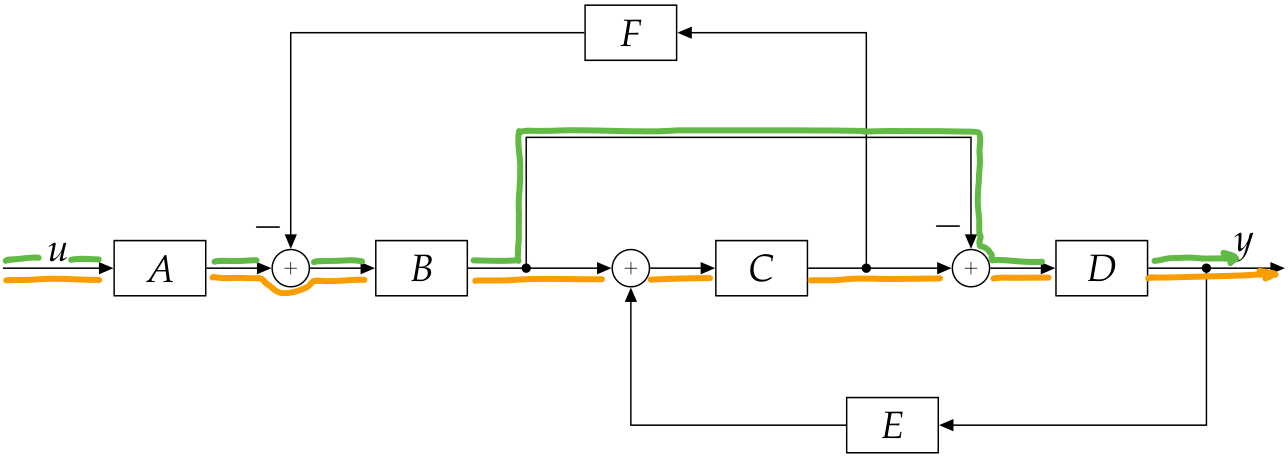
\includegraphics{images/paste-9.png}

}

\end{figure}

\begin{figure}[H]

{\centering 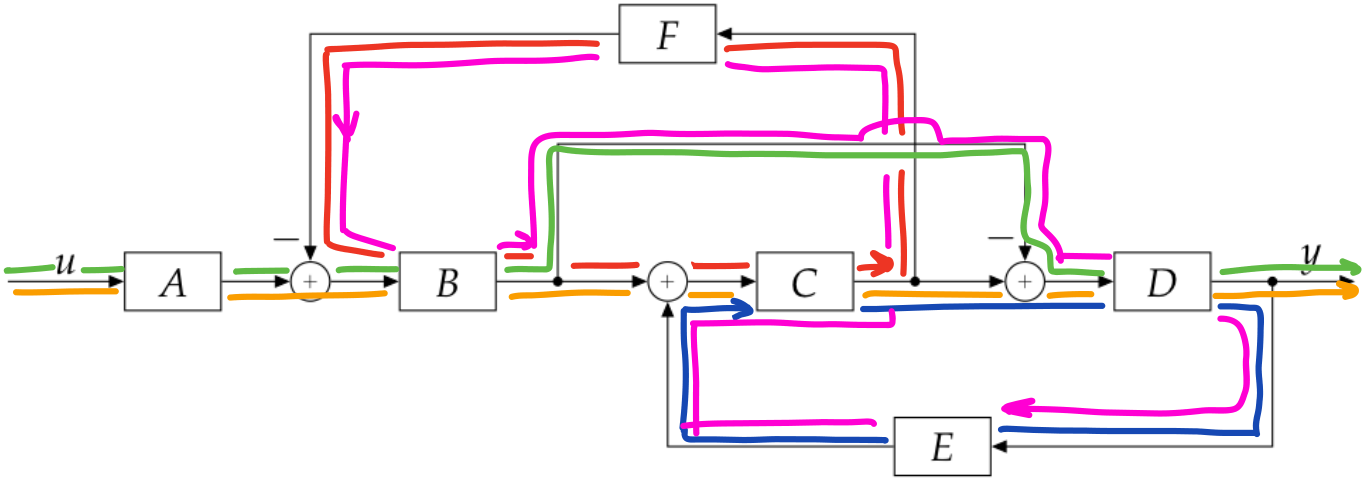
\includegraphics{images/paste-10.png}

}

\end{figure}

\(P_1 = ABCD \quad \Delta_1 = 1-0\quad P_2 = ABD \quad \Delta_2=1-0\)

\(\Delta=A-((-BCF)+CDE+((-B)(-D)(CEF))\)

\[
G_{uy}=\frac{ABD(1+C)}{A+BCF-CDE-BCDEF}
\]

\hypertarget{zustandraumdarstellung}{%
\subsection{Zustandraumdarstellung}\label{zustandraumdarstellung}}

Die Zustandsraumdarstellung erlaubt ein Einblick in das Verhalten eines
dynamischen Systems. Anhand eines \emph{Zeitdiagrammes} und
\emph{Phasenporträit} kann das System \emph{visualisiert} werden. Man
gibt Startkonditionen an und kann über das Phasenporträit den zeitlichen
Verlauf verfolgen.

\begin{figure}[H]

{\centering 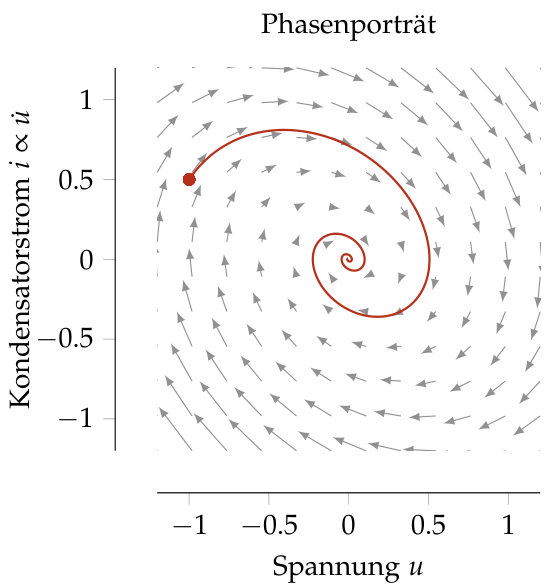
\includegraphics[width=5.7cm,height=\textheight]{images/state_space/quiver.png}

}

\end{figure}

\begin{figure}[H]

{\centering 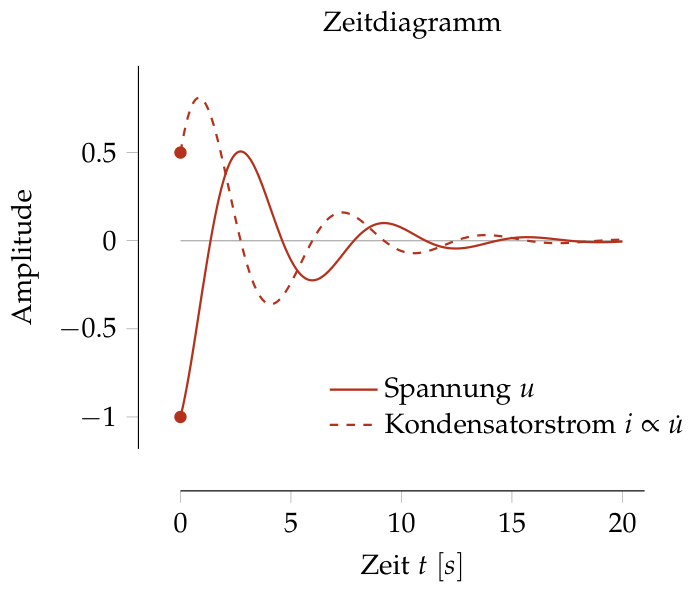
\includegraphics[width=6.3cm,height=\textheight]{images/state_space/time.png}

}

\end{figure}

\hypertarget{autonomes-zeitinvariantes-system}{%
\subsubsection{Autonomes, zeitinvariantes
System}\label{autonomes-zeitinvariantes-system}}

\begin{center}
  \begin{tikzpicture}
    \node[rectangle, draw=black, minimum width = 2cm] (a) at (0,0) {$\frac{dx}{dt} = f(x)$};
    \node (b) at (2,0) {};
    \draw[->] (a) -- node [above] {$x$} (b);
  \end{tikzpicture}
\end{center}

\[
\frac{dx}{dt}=f(x)
\]

Autonome Systeme berücksichtigen äusserliche Beeinflussungen \ul{nicht}
und sind ausschliesslich vom Anfangszustand abhängig.

\hypertarget{allgemeine-systeme}{%
\subsubsection{Allgemeine Systeme}\label{allgemeine-systeme}}

\begin{center}\begin{tikzpicture}

\node[rectangle, draw=black, minimum width = 2cm] (a) at (0,0) {
$
\begin{matrix}
\frac{dx}{dt} = f(x,u) \\
y=h(x,u)
\end{matrix}
$
};
\node (b) at (2,0) {};
\node (c) at (-2,0) {};

\draw[->] (a) -- node [above] {$y$} (b);
\draw[->] (c) -- node [above] {$u$} (a);

\end{tikzpicture}\end{center}

\[
\frac{dx}{dt}=f(x,u)\qquad y=h(x,u)
\]

\hypertarget{lineares-zustandsraummodell}{%
\subsubsection{Lineares
Zustandsraummodell}\label{lineares-zustandsraummodell}}

Viele der Systeme können an ein zeitinvariantes und lineares System
(LTI-System) angenähert werden.

\begin{center}\begin{tikzpicture}[scale=0.8]



\node (entry) at (-1,0) {$u$};
\node[rectangle, draw=black, minimum width=1cm] (integ) at (3.25,0) {$\int{dt}$};
\node[circle, draw=black] (circA) at (3.25,-1) {\textcolor{NavyBlue}{\textbf{A}}};
\node[circle, draw=black] (circB) at (1,0) {\textcolor{BurntOrange}{\textbf{B}}};
\node[sum] (add)   at (2,0) {+};
\node[sum] (add2) at (6.5,0) {+};
\node[circle, draw=black] (circC) at (5.5,0) {\textcolor{BrickRed}{\textbf{C}}};
\node[circle, draw=black] (circD) at (3.25,1) {\textcolor{OliveGreen}{\textbf{D}}};
\node [dot] (v2) at (4.5,0) {};
\node [dot] (v3) at (0,0) {};
\node (end) at (7.5,0) {$y$};


\draw [->] (integ) edge node [above]{$x$} (v2);
\draw [->] (v2) edge (circC);
\draw [->] (add) edge node[above]{$\dot{x}$} (integ);
\draw [->] (circB) edge (add);
\draw [->] (entry) edge (circB);
\draw [->] (circA) -| (add);
\draw [->] (v2) |- (circA);
\draw [->] (v3) |- (circD);
\draw [->] (circD) -| (add2);
\draw [->] (circC) -- (add2);
\draw [->] (add2) -- (end);
\end{tikzpicture}\end{center}

\[
\frac{dx}{dt}=\left(\begin{matrix} \dot{x}_1 \\ \dot{x}_2 \end{matrix}\right)=\textcolor{NavyBlue}{\mathbf{A}}x+\textcolor{BurntOrange}{\mathbf{B}}u \qquad y = \textcolor{BrickRed}{\mathbf{C}}x + \textcolor{OliveGreen}{\mathbf{D}}u
\]

\begin{conditions}
  A & beschreibt Dynamik \\
  B & beschreibt Steuereinfluss \\
  C & beschreibt Messung \\
  D & beschreibt Durchgriff
\end{conditions}

\hypertarget{uxfcbertragungsfunktion}{%
\subsubsection{Übertragungsfunktion}\label{uxfcbertragungsfunktion}}

Wird als Eingangssignal \(u\)

\[
u=\cos(\omega t)=\frac12(e^{+j\omega t}+e^{-j\omega t})
\]

gegeben, ergibt sich folgendes Ausgangssignal

\[
y(t)=\underbrace{C\textcolor{BrickRed}{e^{At}}(x(0)-(sI-A)^{-1}B)}_{\text{transient } y_t} + \underbrace{\overbrace{(C(sI-A)^{-1}B+D)}^{\text{Übertragungsfunktion}} e^{st}}_{\text{stationär } y_s}
\]

\begin{tcolorbox}[enhanced jigsaw, leftrule=.75mm, opacityback=0, left=2mm, arc=.35mm, breakable, coltitle=black, rightrule=.15mm, opacitybacktitle=0.6, titlerule=0mm, title=\textcolor{quarto-callout-note-color}{\faInfo}\hspace{0.5em}{Hinweis}, bottomtitle=1mm, colbacktitle=quarto-callout-note-color!10!white, colframe=quarto-callout-note-color-frame, colback=white, bottomrule=.15mm, toptitle=1mm, toprule=.15mm]

Ist \(A\) stabil, so geht der transiente Anteil \(y_t\) asymptotisch
gegen Null. Der stationäre Anteil bleibt übrig und entspricht der
Übertragungsfunktion.

\end{tcolorbox}

\hypertarget{the-z-transform}{%
\section{The z-Transform}\label{the-z-transform}}

\begin{figure}[H]

{\centering 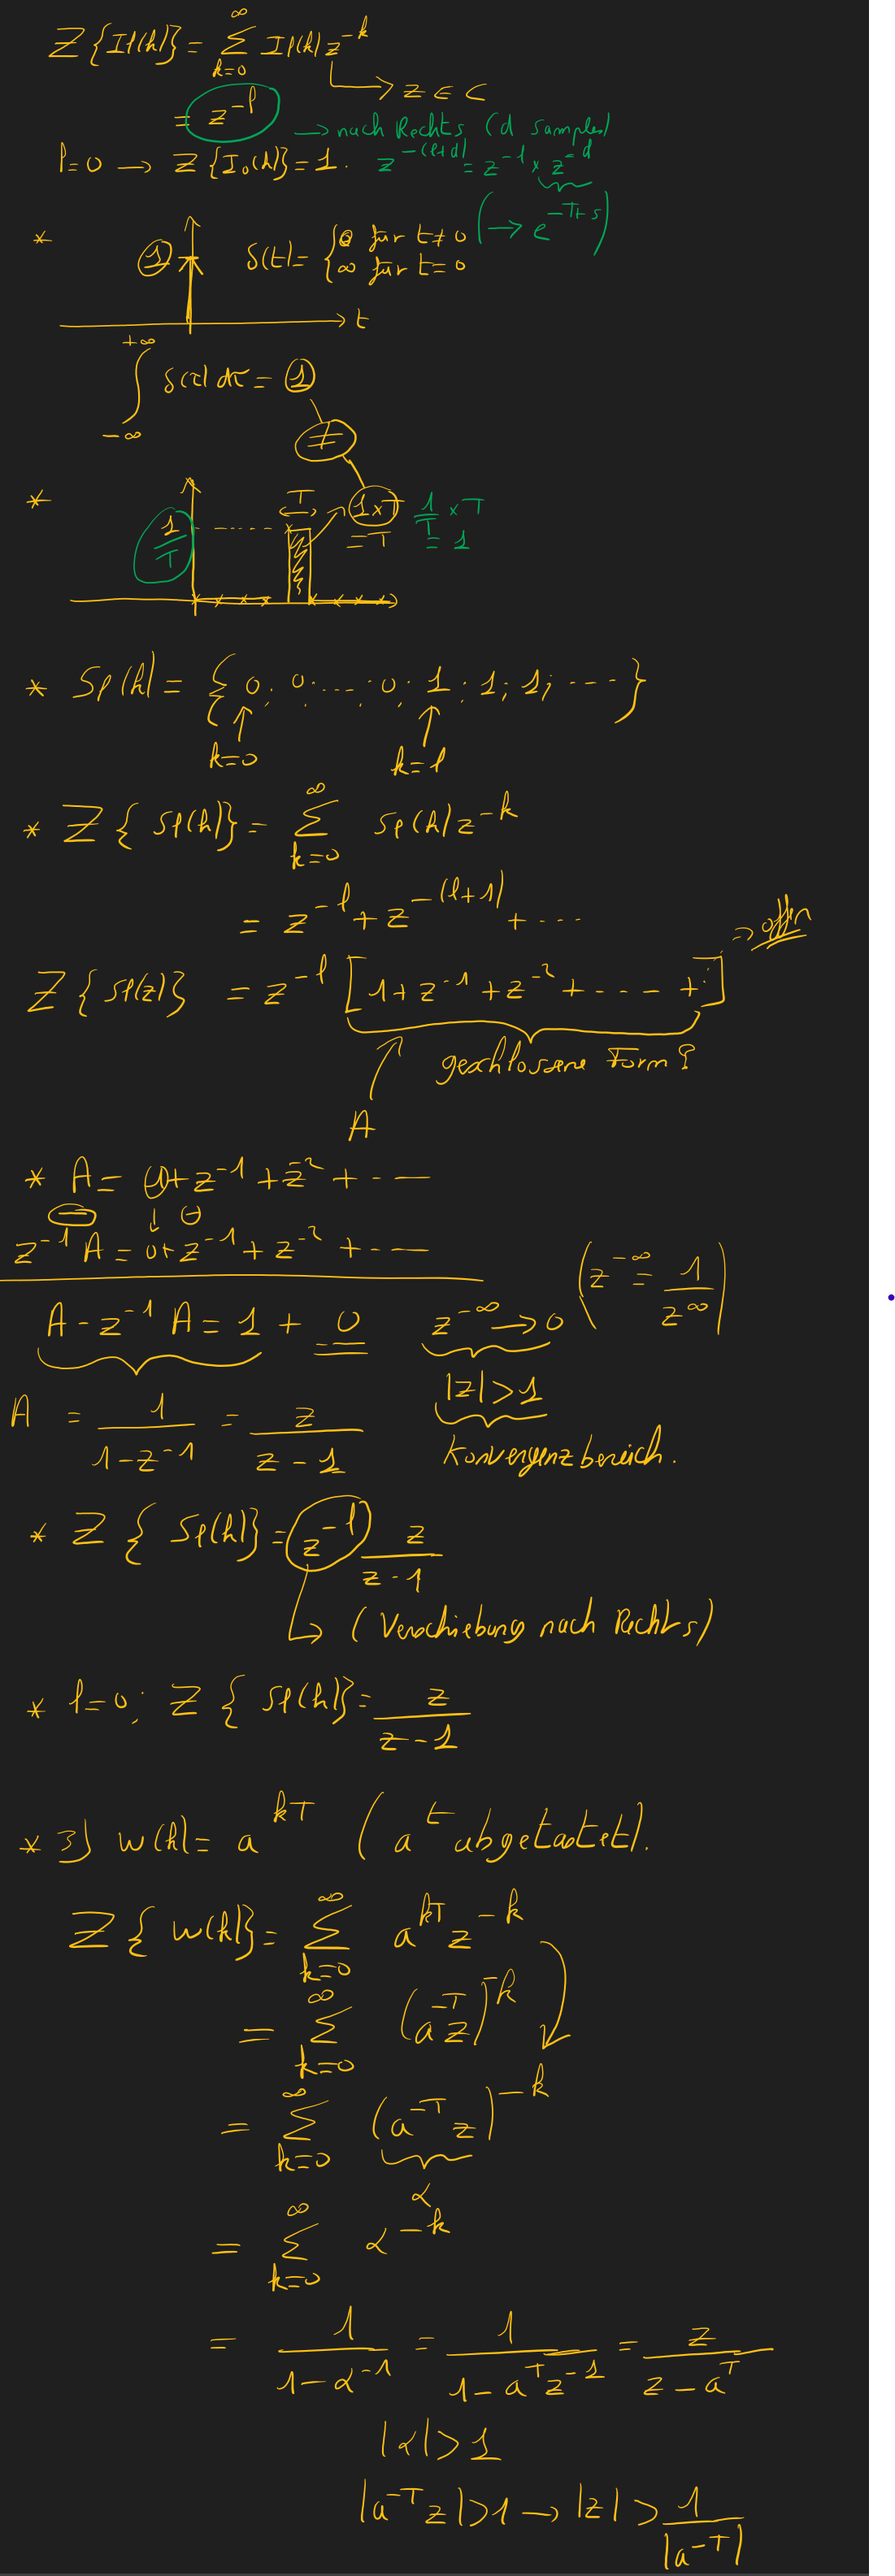
\includegraphics{images/IAS/Z-Transformation.png}

}

\end{figure}

\hypertarget{diskreten-regelkreis}{%
\section{diskreten Regelkreis}\label{diskreten-regelkreis}}

\begin{figure}[H]

{\centering 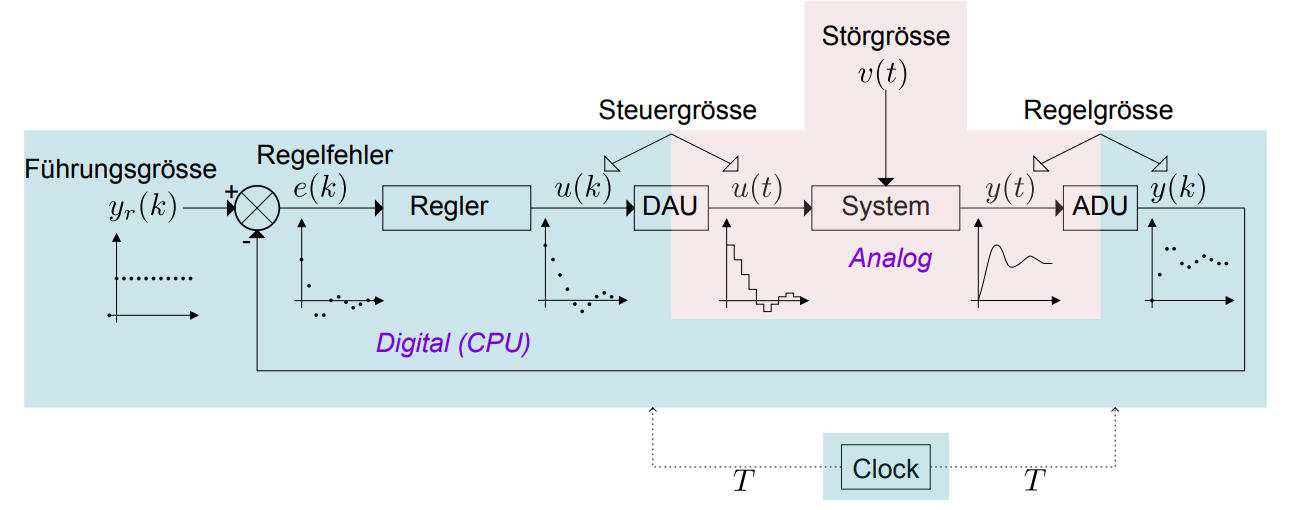
\includegraphics{images/IAS/snip1.png}

}

\end{figure}

\hypertarget{p-anteil}{%
\subsection{P-Anteil}\label{p-anteil}}

\begin{longtable}[]{@{}
  >{\raggedright\arraybackslash}p{(\columnwidth - 2\tabcolsep) * \real{0.4340}}
  >{\raggedright\arraybackslash}p{(\columnwidth - 2\tabcolsep) * \real{0.5660}}@{}}
\toprule\noalign{}
\endhead
\bottomrule\noalign{}
\endlastfoot
\(                    
 P = u(t) = k_p * e(k)  
 \) & 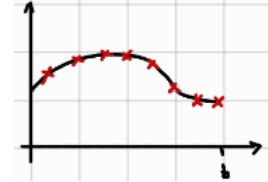
\includegraphics{images/IAS/P-Anteil.png} \\
\end{longtable}

\hypertarget{i-anteil}{%
\subsection{I-Anteil}\label{i-anteil}}

Beim I -- Anteil gibt es drei Varianten:

\begin{longtable}[]{@{}
  >{\raggedright\arraybackslash}p{(\columnwidth - 4\tabcolsep) * \real{0.2192}}
  >{\raggedright\arraybackslash}p{(\columnwidth - 4\tabcolsep) * \real{0.5137}}
  >{\raggedright\arraybackslash}p{(\columnwidth - 4\tabcolsep) * \real{0.2603}}@{}}
\toprule\noalign{}
\endhead
\bottomrule\noalign{}
\endlastfoot
Rückwärtsrechteck Regel & \(
u(k) \thickapprox u_i * (k-1) +\frac{k_p}{T_i}*e(k) * T
\) & \includegraphics{images/IAS/I-Anteil-Rück.png} \\
Vorwärtsrechteck Regel &
\( u(k) \thickapprox u_i * (k-1) +\frac{k_p}{T_i}*e(k - 1) * T
\) & 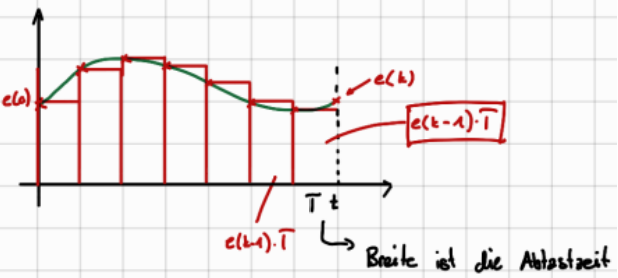
\includegraphics{images/IAS/I-Anteil-Vor.png} \\
Trapez Regel ``Tustin- Approx'' & \(
u(k) \thickapprox u_i * (k-1) +\frac{k_p}{T_i}*\frac{e(k) - e(k-1)}{2}*T
\) & 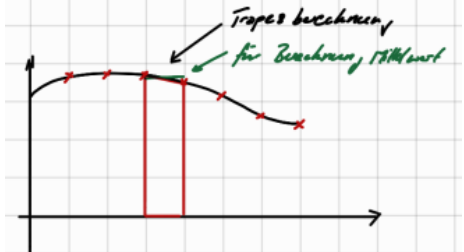
\includegraphics{images/IAS/I-Anteil-Trapez.png} \\
\end{longtable}

\hypertarget{d-anteil}{%
\subsection{D-Anteil}\label{d-anteil}}

\begin{longtable}[]{@{}
  >{\raggedright\arraybackslash}p{(\columnwidth - 2\tabcolsep) * \real{0.6429}}
  >{\raggedright\arraybackslash}p{(\columnwidth - 2\tabcolsep) * \real{0.3571}}@{}}
\toprule\noalign{}
\endhead
\bottomrule\noalign{}
\endlastfoot
\(                                                   
 u_d \thickapprox k_p * T_d * \frac{e(k) - e(k-1)}{T}  
 \) & 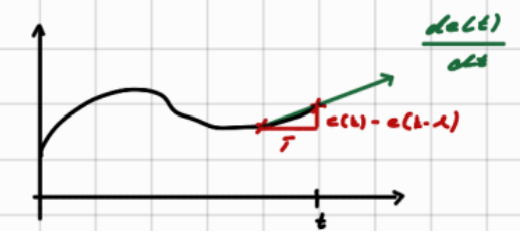
\includegraphics{images/IAS/D-Anteil.png} \\
\end{longtable}



\end{document}
